  Detectors section
\subsection{SiD Detector - Introduction}
The SiD detector is a general-purpose experiment designed to perform precision measurements
at ILC. It satisfies the challenging detector requirements resulting from the full range of ILC physics processes. SiD is based on the paradigm of particle flow, an algorithm by which
the reconstruction of both charged and neutral particles is accomplished by an optimised
combination of tracking and calorimetry. The net result is a significantly more precise jet
energy measurement which results in a di-jet mass resolution good enough to distinguish
between W’s and Z’s.
The SiD detector (Fig.~\ref{fig:fig_sid})is a compact detector based on a powerful silicon
pixel vertex detector, silicon tracking, silicon-tungsten electromagnetic calorimetry and
highly segmented hadronic calorimetry. SiD also incorporates a high-field solenoid, iron
flux return, and a muon identification system. The use of silicon sensors in the vertex, tracking
and calorimetry enables a unique integrated tracking system ideally suited to particle
flow.
The choice of silicon detectors for tracking and vertexing ensures that SiD is robust
with respect to beam backgrounds or beam loss, provides superior charged particle momentum
resolution, and eliminates out-of-time tracks and backgrounds. The main tracking
detector and calorimeters are “live” only during a single bunch crossing, so beam-related
backgrounds and low-pT backgrounds from \gamgam processes will be reduced to the minimum
possible levels. The SiD calorimetry is optimised for excellent jet energy measurement
using the particle flow technique. The complete tracking and calorimeter systems are contained
within a superconducting solenoid, which has a 5 T field strength, enabling the overall
compact design. The coil is located within a layered iron structure that returns the magnetic flux and is instrumented to allow the identification of muons. All aspects of SiD are the result of intensive and leading-edge research aimed at achieving
performance at unprecedented levels. At the same time, the design represents a balance between cost
and physics performance. The key parameters of the SiD design are listed in  Table~\ref{sid:ConceptOverview:Table:Ovw_sidparams}.

\begin{figure}[tb]
 %\epsfysize=9.0cm
 \begin{center}
 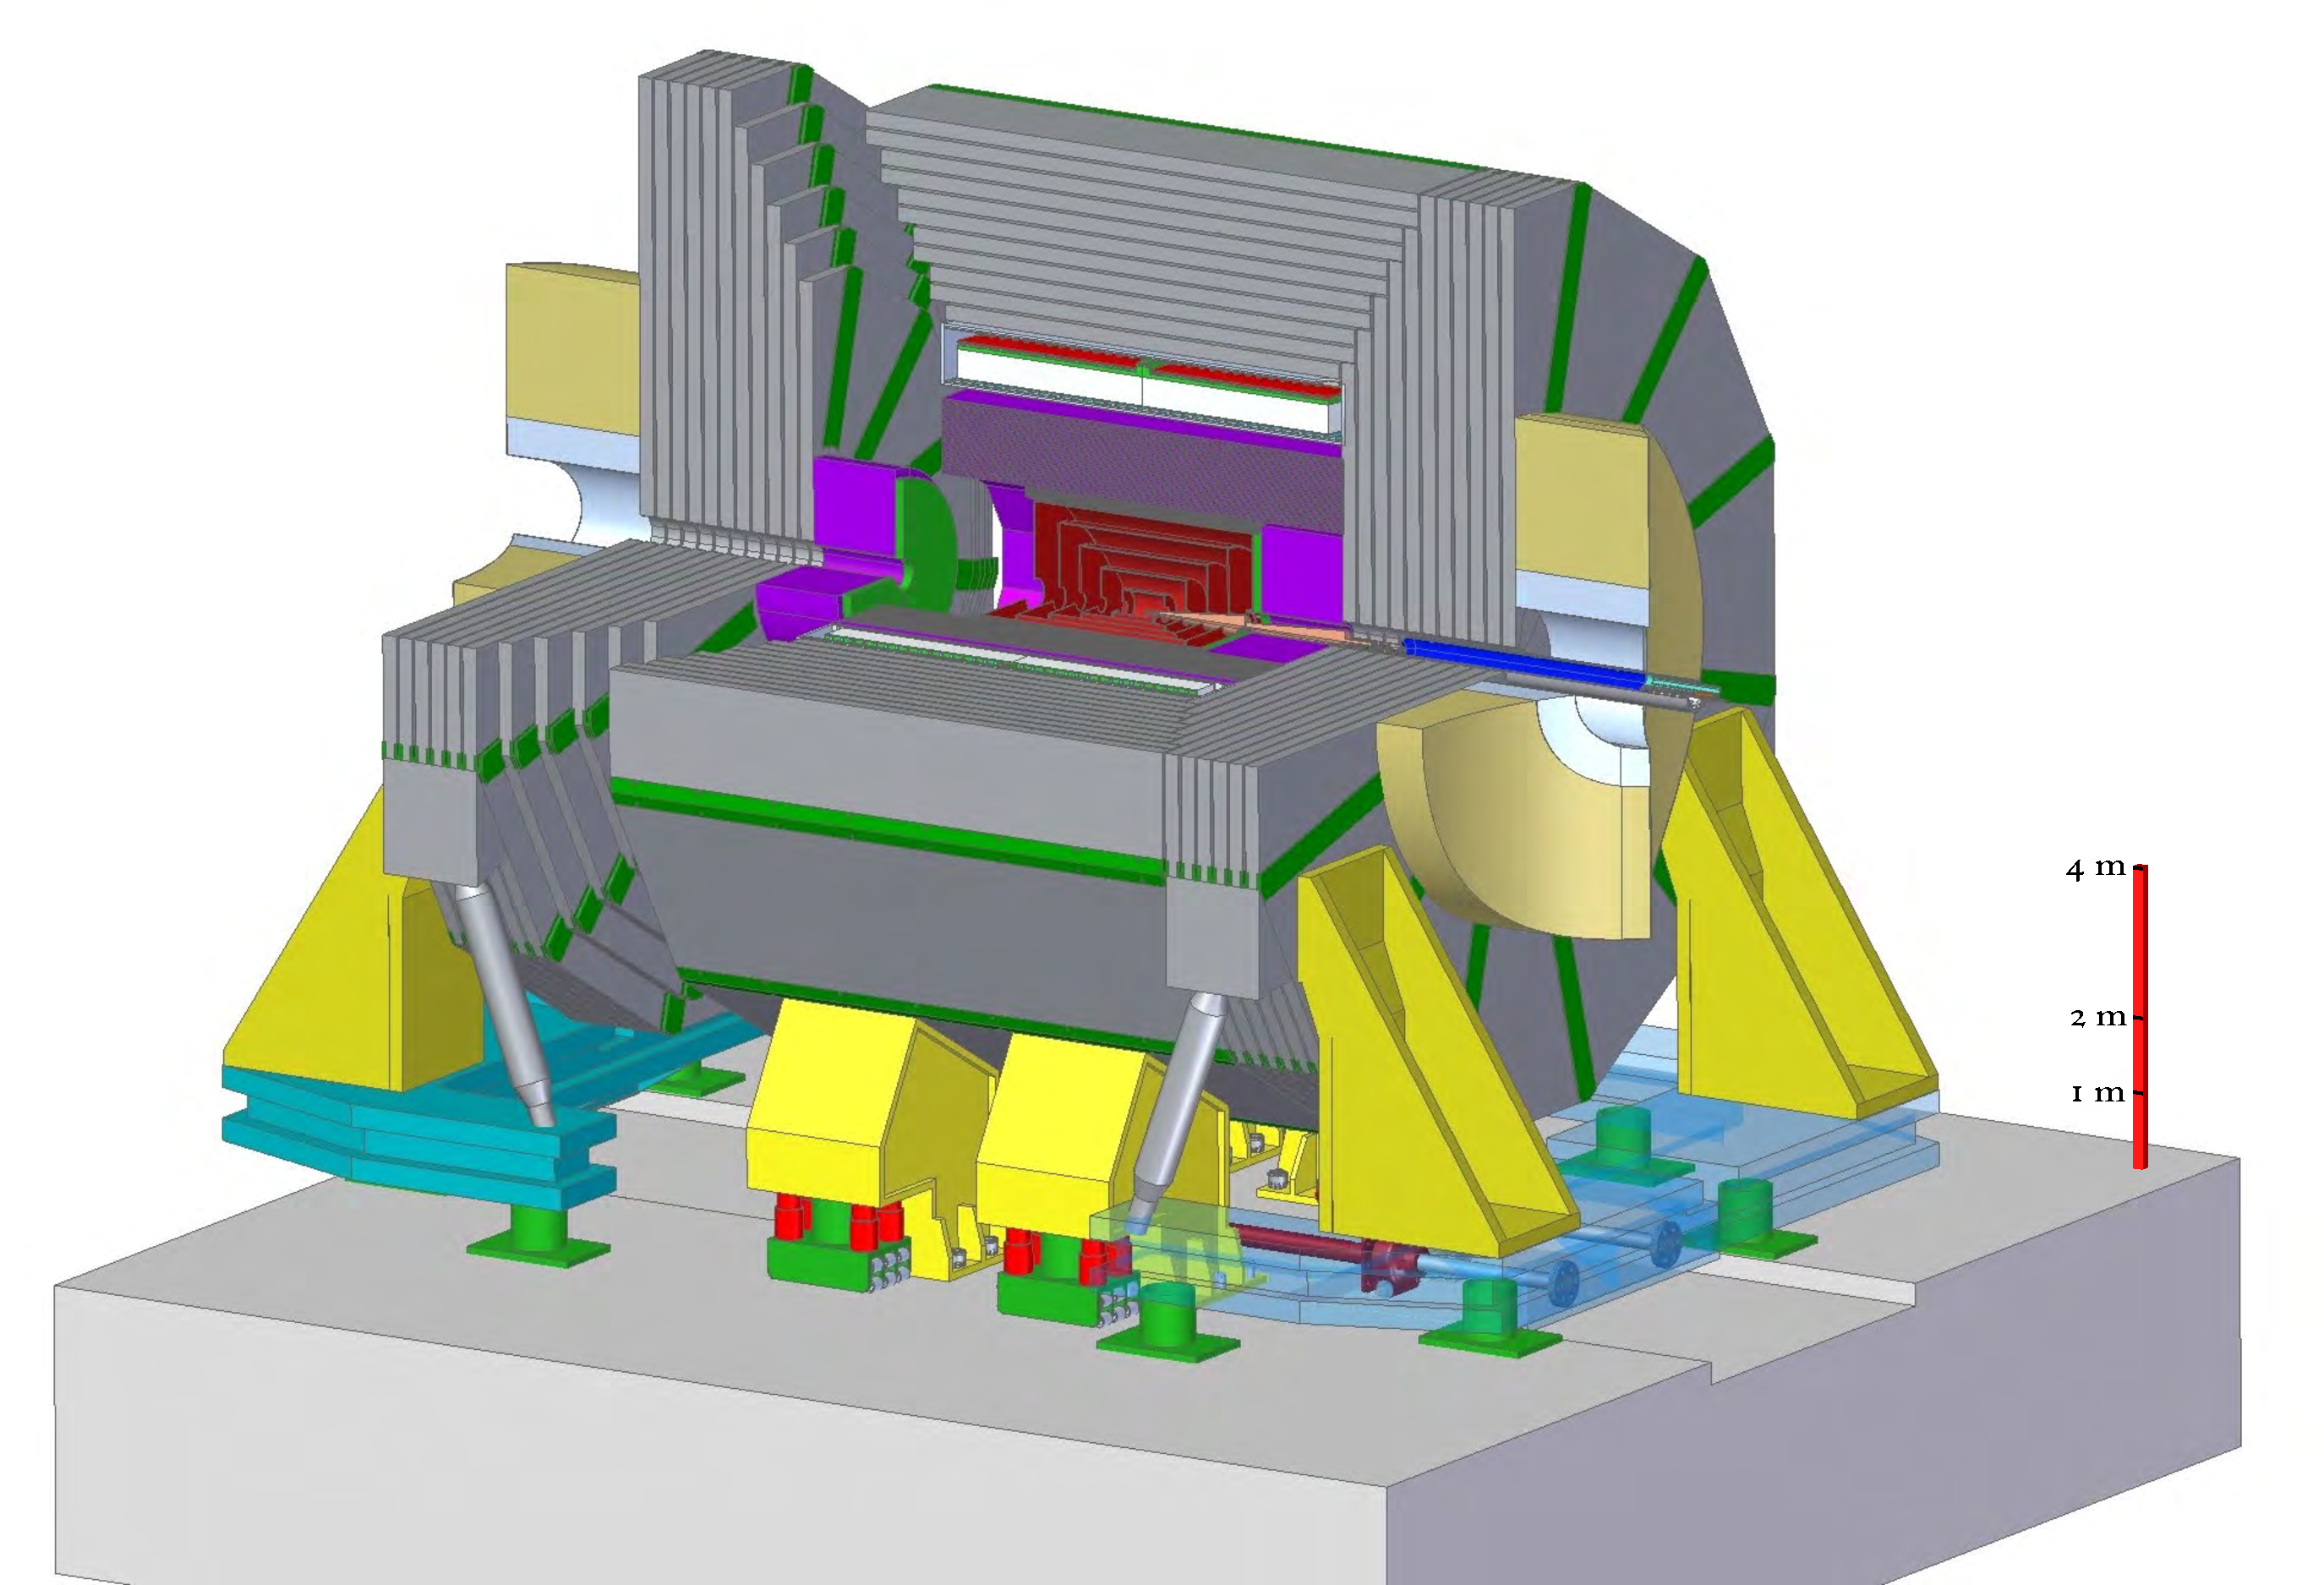
\includegraphics[width=0.9\hsize]{chapters/figures/SiD.pdf}
\caption{The SiD detector concept.
\label{fig_sid}}
 \end{center}
 \vspace{-0.7cm}
 \end{figure}

\thisfloatsetup{floatwidth=\SfigwFull,capposition=beside}
\begin{table}[htbp]
\renewcommand{\arraystretch}{1.25}

\ttabbox{

\caption{\label{sid:ConceptOverview:Table:Ovw_sidparams}Key parameters of the baseline \sid design. (All dimension
are given in cm).}
}
{
\begin{tabular}{l l r r r}
    \toprule
    \sid Barrel& Technology& Inner radius& Outer radius& z extent \\
    \midrule
    Vertex detector& Silicon pixels& 1.4& 6.0& $\pm \quad 6.25$ \\
    Tracker& Silicon strips& 21.7& 122.1& $\pm \quad 152.2$ \\
    ECAL& Silicon pixels-W& 126.5& 140.9& $\pm \quad 176.5$ \\
    HCAL& RPC-steel& 141.7& 249.3& $\pm \quad 301.8$ \\
    Solenoid& 5 Tesla SC & 259.1& 339.2& $\pm \quad 298.3$ \\
    Flux return& Scintillator-steel& 340.2 & 604.2& $\pm \quad 303.3$ \\
    \bottomrule

   \toprule
 \sid Endcap& Technology& Inner z& Outer z& Outer radius \\
    \midrule
Vertex detector& Silicon pixels& 7.3& 83.4& 16.6 \\
Tracker& Silicon strips& 77.0& 164.3& 125.5 \\
ECAL& Silicon pixel-W& 165.7& 180.0& 125.0 \\
HCAL& RPC-steel& 180.5& 302.8& 140.2 \\
Flux return& Scintillator/steel& 303.3& 567.3& 604.2 \\
LumiCal& Silicon-W& 155.7& 170.0& 20.0 \\
BeamCal& Semiconductor-W& 277.5& 300.7& 13.5 \\
    \bottomrule
\end{tabular}
}

\end{table}

\subsubsection{Silicon-based Tracking}
The tracking system (Fig.~\ref{fig:fig_vxdtrk}) is a key element of the ILC detector concepts. The
particle flow algorithm requires excellent tracking with superb efficiency and
two-particle separation. The requirements for precision measurements, in
particular in the Higgs sector, place high demands on the momentum resolution at
the level of $\delta (1/\pT)  \sim 2-5 \times 10^{-5}/$GeV/$c$.

Highly efficient charged particle tracking is achieved using the pixel detector
and main tracker to recognise and measure prompt tracks, in conjunction with the ECAL, which can
identify short track stubs in its first few layers 
to catch tracks arising from secondary decays of long-lived particles. With
the choice of a 5~T solenoidal magnetic field, in part chosen to control the \epem pair
background, the design allows for a compact tracker design. 

\begin{figure}[tb]
 %\epsfysize=9.0cm
 \begin{center}
 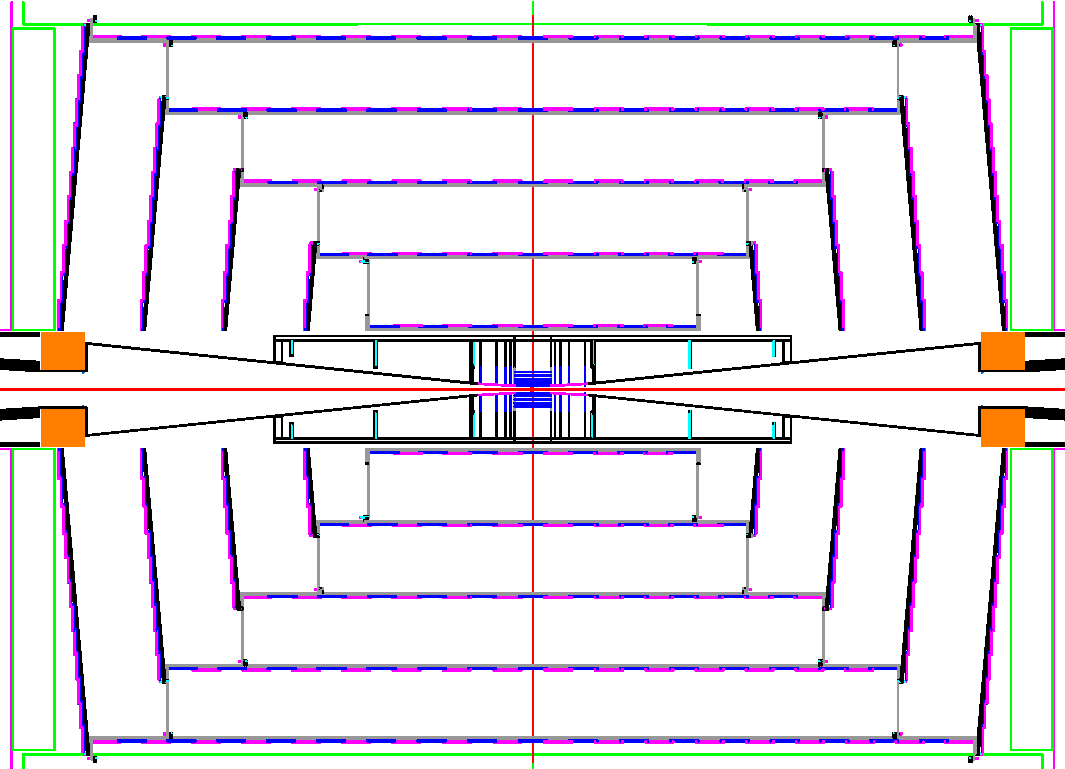
\includegraphics[width=0.9\hsize]{chapters/figures/vxdtrk.pdf}
\caption{r-z view of vertex detector and outer tracker.
\label{fig_vxdtrk}}
 \end{center}
 \vspace{-0.7cm}
 \end{figure}

\subsubsection{Vertex detector}

To unravel the underlying physics mechanisms of new observed processes, the
identification of heavy flavours will play a critical role. One of the main
tools for heavy flavour identification is the vertex detector. The physics goals
dictate an unprecedented spatial three-dimensional point resolution and a very
low material budget to minimise multiple Coulomb scattering. The running 
conditions at the ILC impose the readout speed and radiation tolerance. 
These requirements are normally in tension. High
granularity and fast readout compete with each other and tend to increase the
power dissipation. Increased power dissipation in turn leads to an increased
material budget. The challenges on the vertex detector are considerable and
significant R\&D is being carried out on both the development of the sensors and
the mechanical support.
The \sid vertex detector uses a barrel and disk layout. The barrel section
consists of five silicon pixel layers with a pixel size of
$20~\times~20~\micron^2$. The forward and backward regions each have four
silicon pixel disks. In addition, there are three silicon pixel disks at a
larger distance from the interaction point to provide uniform coverage for the
transition region between the vertex detector and the outer tracker. This
configuration provides for very good hermeticity with uniform coverage and
guarantees excellent charged-track pattern recognition capability and impact parameter resolution 
over the full solid angle. 
This enhances the capability of the integrated tracking system and, 
in conjunction with the high magnetic field, makes for a very compact
system, thereby minimising the size and costs of the calorimetry.

To provide for a very robust track-finding performance the baseline 
choice for the vertex detector has a sensor technology that provides
time-stamping of each hit with sufficient precision to assign it to
a particular bunch crossing. This significantly suppresses
backgrounds. 

Several technologies are being developed. One of them is a CMOS-based
monolithic pixel sensor called Chronopixel. The main goal for the design is a
pixel size of about $10~\times~10~\micron^2$ with 99\% charged-particle
 efficiency. Prototype devices have demonstrated that the concept works; 
what should be a fully functional chip is presently under test. More 
challenging is the 3D vertical integrated silicon technology, for which a full 
demonstration is also close.

Minimising the support material is critical to the development of a high-performance 
vertex detector. An array of 
low-mass materials such as reticulated foams and silicon-carbide
materials are under consideration. An alternative approach that is being pursued very actively is the
embedding of thinned, active sensors in ultra low-mass media. This line of R\&D
explores thinning active silicon devices to such a thickness that the silicon
becomes flexible. The devices can then be embedded in, for example, Kapton
structures, providing extreme versatility in designing and constructing a vertex
detector.

Power delivery must be accomplished without exceeding the material budget and
over heating the detector.  The vertex detector 
design relies on power pulsing during bunch trains to minimise heating 
and uses forced air for cooling. 

\subsubsection{Main tracker}
The main tracker technology of
choice is silicon strip sensors arrayed in five nested cylinders in the central
region and four disks following a conical surface with an angle of 5 degrees
with respect to the normal to the beamline in each of the end regions. The geometry of the endcaps
minimises the material budget to enhance forward tracking. The detectors are
single-sided silicon sensors, approximately 10 $\times$ 10 cm$^2$ with a readout
pitch of 50~\micron. The endcaps utilise two sensors bonded back-to-back for
small angle stereo measurements. With an outer cylinder radius of 1.25~m
and a 5~T field, the charged track momentum resolution will be better than
$\delta (1/\pT) = 5 \times 10^{-5} $/(GeV/$c$) for high momentum tracks with coverage down to polar angles of 10 degrees.

The all-silicon tracking approach has been extensively tested using full Monte-Carlo
simulations including full beam backgrounds. Besides having an excellent momentum resolution
it provides robust pattern recognition even in the presence of backgrounds and has a
real safety margin, if the machine backgrounds will be worse than expected.

\subsubsection{Main calorimeters}

The \sid baseline design incorporates the elements needed to
successfully implement the PFA approach. This imposes a number of
basic requirements on the calorimetry. The central calorimeter
system must be contained within the solenoid in order to reliably associate
tracks to energy deposits. The electromagnetic and hadronic sections
must have imaging capabilities that allow both efficient
track-following and correct assignment of energy clusters to tracks. These
requirements imply that the calorimeters must be finely segmented both
longitudinally and transversely. In order to ensure that no significant amount
of energy can escape detection, the calorimetry must extend down to small
angles with respect to the beampipe and must be sufficiently deep to prevent
significant energy leakage. Since the average penetration depth of a hadronic
shower grows with its energy, the calorimeter system must be designed for the
highest-energy collisions envisaged.

In order to ease detector construction the calorimeter mechanical design consists of a series of modules of
manageable size and weight. The boundaries between
modules are kept as small as possible to prevent significant non-instrumented
regions. The detectors are designed to have excellent long-term stability and reliability,
since access during the data-taking period will be extremely limited, if not
impossible.

The combined ECAL and HCAL systems consist of a
central barrel part and two endcaps, nested inside the barrel. The entire barrel system is contained
within the volume of the cylindrical superconducting solenoid. 

The
electromagnetic calorimeter has silicon active layers between tungsten absorber
layers. The active layers use 5$\times$5~mm$^2$ silicon pixels, which provide excellent spatial resolution.
The structure has 30 layers in total, the first 20 layers having a
thinner absorber than the last ten layers. This configuration is a 
compromise between cost, electromagnetic shower radius, sampling frequency, and
shower containment. The total depth of the electromagnetic calorimeter is 26
radiation lengths (\xo) and one nuclear interaction length. 

The hadronic
calorimeter has a depth of 4.5 nuclear interaction lengths, consisting of
alternating steel plates and active layers. The baseline choice for the active
layers is scintillator tiles read out via silicon photomultipliers. For this approach SiD is closely following the analog hadron calorimeter developments within the CALICE collaboration.

\subsubsection{Forward calorimeters}

Two special calorimeters are foreseen in the very forward region: LumiCal for precise measurement, and BeamCal for fast
estimation, of the luminosity. LumiCal and BeamCal are
compact cylindrical electromagnetic calorimeters centred on the outgoing beam.
They are based on 30 layers' depth of semiconductor-tungsten technology. BeamCal
is placed just in front of the final focus quadrupole and LumiCal is aligned
with the electromagnetic calorimeter endcap. LumiCal uses silicon sensor readout.
It is a precision device with
challenging requirements on the mechanics and position control. BeamCal is
exposed to a large flux of low-energy electron-positron pairs originating from
beamstrahlung. These depositions, useful for a bunch-by-bunch luminosity
estimate and the determination of beam parameters, require radiation hard
sensors. The detectors in the very forward region have to tackle relatively high
occupancies, requiring dedicated front-end electronics.

The challenge for BeamCal is to find sensors that will tolerate about one MGy
of dose per year. So far polycrystalline chemical vapour deposition (CVD) diamond
sensors of area 1~cm$^2$ and larger sectors of GaAs pad sensors have been studied. Since
large-area CVD diamond sensors are extremely expensive, they may be used for only
the innermost part of BeamCal. At larger radii GaAs sensors appear to be a
promising option. Sensor samples produced using the liquid encapsulated
Czochralski method have been studied in a high-intensity electron beam. 

For SiD,
the main activities are the study of these radiation-hard sensors, development
of the first version of the so-called Bean readout chip, and the simulation of BeamCal
tagging for physics studies. SiD coordinates these activities with the FCAL R\&D Collaboration. 

\subsubsection{Magnet Coil}

The \sid superconducting solenoid is based on the CMS solenoid
design philosophy and construction techniques, using a slightly modified CMS
conductor as its baseline design. Superconducting strand count in the coextruded
Rutherford cable was increased from 32 to 40 to accommodate the higher 5~T
central field. 

Many iron flux return configurations have been simulated in two
dimensions so as to reduce the fringe field. An Opera 3D calculation with the Detector
Integrated Dipole (DID) coil has been completed.
Calculations of magnetic field with a 3D ANSYS program
are in progress. These will have the capability to calculate forces and stress
on the DID as well as run transient cases to check the viability of using the
DID as a quench propagator for the solenoid. Field and force calculations with
an iron endcap HCAL were studied. The field homogeneity improvement was found
to be insufficient to pursue this option. 

Conceptual DID construction and
assembly methods have been studied. The solenoid electrical power system,
including a water-cooled dump resistor and grounding, was established.
Significant work has been expended on examining different conductor stabiliser
options and conductor fabrication methods. This work is pursued as a cost- and
time-saving effort for solenoid construction.

\subsubsection{Muon System}
The flux-return yoke is instrumented with position sensitive detectors to
serve as both a muon filter and a tail catcher. The total area to be
instrumented is very significant - several thousand square meters. Technologies
that lend themselves to low-cost large-area detectors are therefore under
investigation. Particles arriving at the muon system have seen large amounts of
material in the calorimeters and encounter significant multiple scattering
inside the iron. Spatial resolution of a few centimetres is therefore
sufficient. Occupancies are low, so strip detectors are possible. The \sid
baseline design uses scintillator technology, with RPCs as an alternative. 
The scintillator technology uses extruded scintillator readout with wavelength 
shifting fibre and SiPMs, and has been successfully demonstrated. 
Simulation studies have shown that nine or more layers of sensitive detectors 
yield adequate energy measurements and good muon-detection efficiency and purity.


\subsubsection{The Machine-Detector Interface}
A time-efficient implementation of the push-pull model of
operation sets specific requirements and challenges for many detector and
machine systems, in particular the interaction region (IR) magnets, the
cryogenics, the alignment system, the beamline shielding, the detector design
and the overall integration. The minimal functional requirements and interface
specifications for the push-pull IR have been successfully developed and
published~\cite{Platform_Agreement,IR_Layout}, to which all further IR design
work on both the detectors and machine sides are constrained.

\subsection{The ILD Detector}
The ILD detector is a proposed detector for the international linear collider, ILC. It has been developed by a proto-collaboration with the goal to develop and eventually propose a fully integrated detector for the ILC. 

The ILD detector concept has been designed as a multi-purpose detector. It should deliver excellent physics performance for collision energies between 90~Gev and 1~TeV, the largest possible energy reach of the ILC. The ILD detector has been optimized to perform excellently at the initial ILC energy of 250 GeV (for more details see \cite{ild:bib:ILDloi}, \cite{ild:bib:ILDDBD}).

The science which will be done at the ILC requires a true multi-purpose detector. A central element of the design has been the capability of the detector to reconstruct precisely complex hadronic final states as well as more events with leptons or missing energy in the final state. Thus traditional precision detector elements as vertex detectors are combined in an overall design philosophy called particle flow, which has been developed for optimal hadronic event reconstruction.

The high precision vertex detector positioned very closely to the interaction point is followed by a hybrid tracking layout, realised as a combination of silicon tracking with a time projection chamber, and a calorimeter system. The complete system is located inside a large solenoid providing a magnetic field of 3.5-4 T. On the outside of the coil, the iron return yoke is instrumented as a muon system and as a tail catcher calorimeter. 

The vertex detector is realised as a multi-layer pixel-vertex detector (VTX), with three super-layers each comprising two layers. The detector has a pure barrel geometry. To minimise the occupancy from background hits,
the first super-layer is only half as long as the outer two. Whilst the underlying detector technology has not yet been decided, 
the VTX is optimised for point resolution and minimum material thickness. 
	
A system of silicon strip and pixel detectors surrounds the VTX detector. In the barrel, two layers of silicon strip detectors (SIT) are arranged to bridge the gap between the VTX and the TPC. In the forward region, a system of two silicon-pixel disks and five silicon-strip disks (FTD) provides low angle tracking coverage.

A distinct feature of ILD is a large volume time projection chamber (TPC) with up to 224 points per track. The TPC is optimised for 3-dimensional point resolution and minimum material in the field cage and in the end-plate. It also allows d$E$/d$x$ based particle identification. At the ILC a TPC has a number of specific strength, which make this type of detector attractive. A time projection chamber offers true three-dimensional points, and offers many of those along a charged particle trajectory. The intrinsic disadvantage of a TPC, its slow readout speed, does not really harm the performance at the ILC, since the time between bunches is relativly long, with around 300~ns. On the other hand the large number of points offer superb pattern recognition capabilities, and allows the detailed reconstruction of kinks or decays in flight within its volume. This can be achieved at a very low material budget, rather uniforly distributed over the sensitive volume. The excellent performance of the system is particularly striking at low momenta, at a few GeV and below, where the combination of three dimensional reconstruction and low material allows the efficient and precise reconstruction of tracks. 

Outside the TPC a system of Si-strip detectors in between the TPC and the ECAL (SET), provide additional high precision space points which improve the tracking performance and provide additional
    redundancy in the regions between the main tracking volume and the calorimeters. 

A highly segmented electromagnetic calorimeter (ECAL) provides up to 30 samples in depth and small transverse cell size, split into a barrel and an end cap system. For the absorber Tungsten has been chosen, for the sensitive area silicon diodes or scintillator strips are considered.
\thisfloatsetup{floatwidth=\SfigwFull,capposition=beside}
\begin{figure}[t!]
\begin{tabular}{cc}
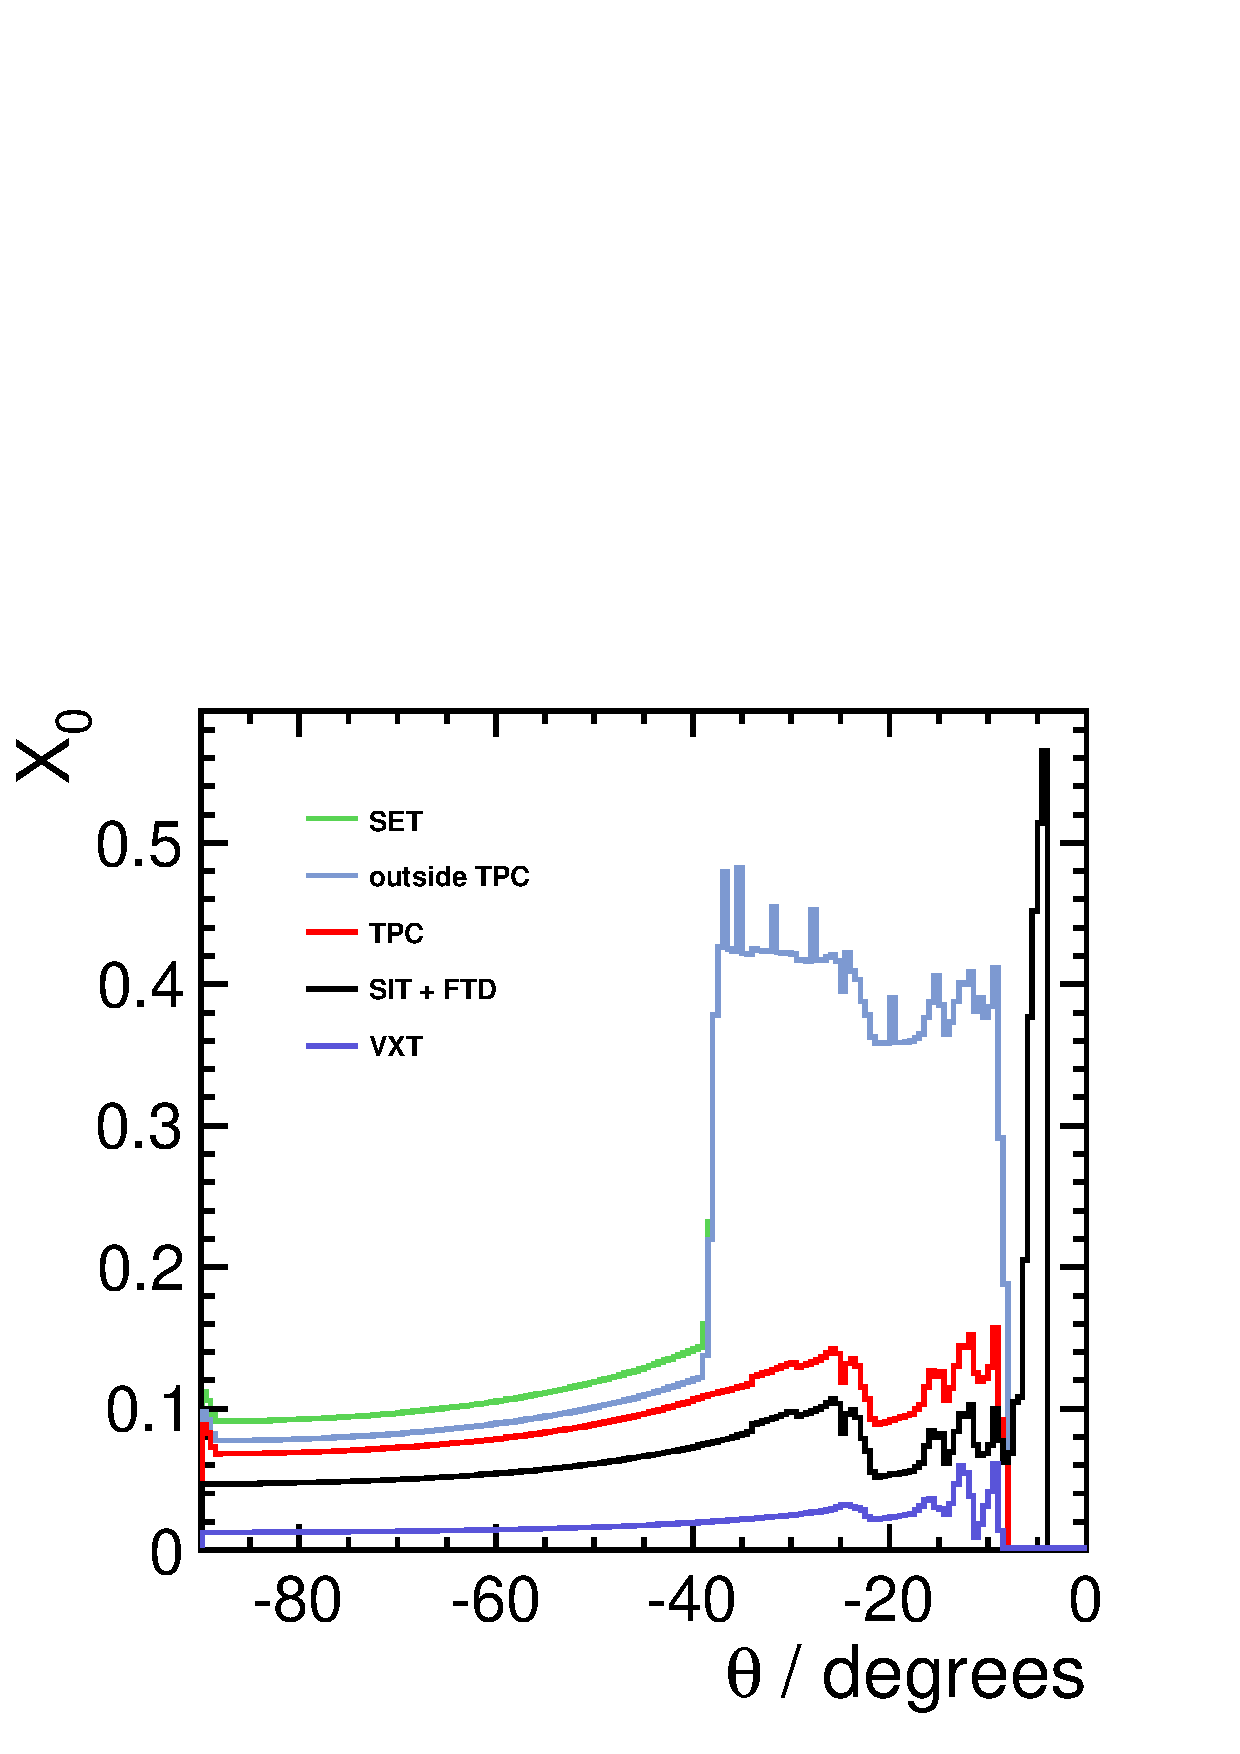
\includegraphics[width=0.52\hsize,viewport={0 -10 600 500},clip]{Introduction/fig/material-budget-new.pdf} &
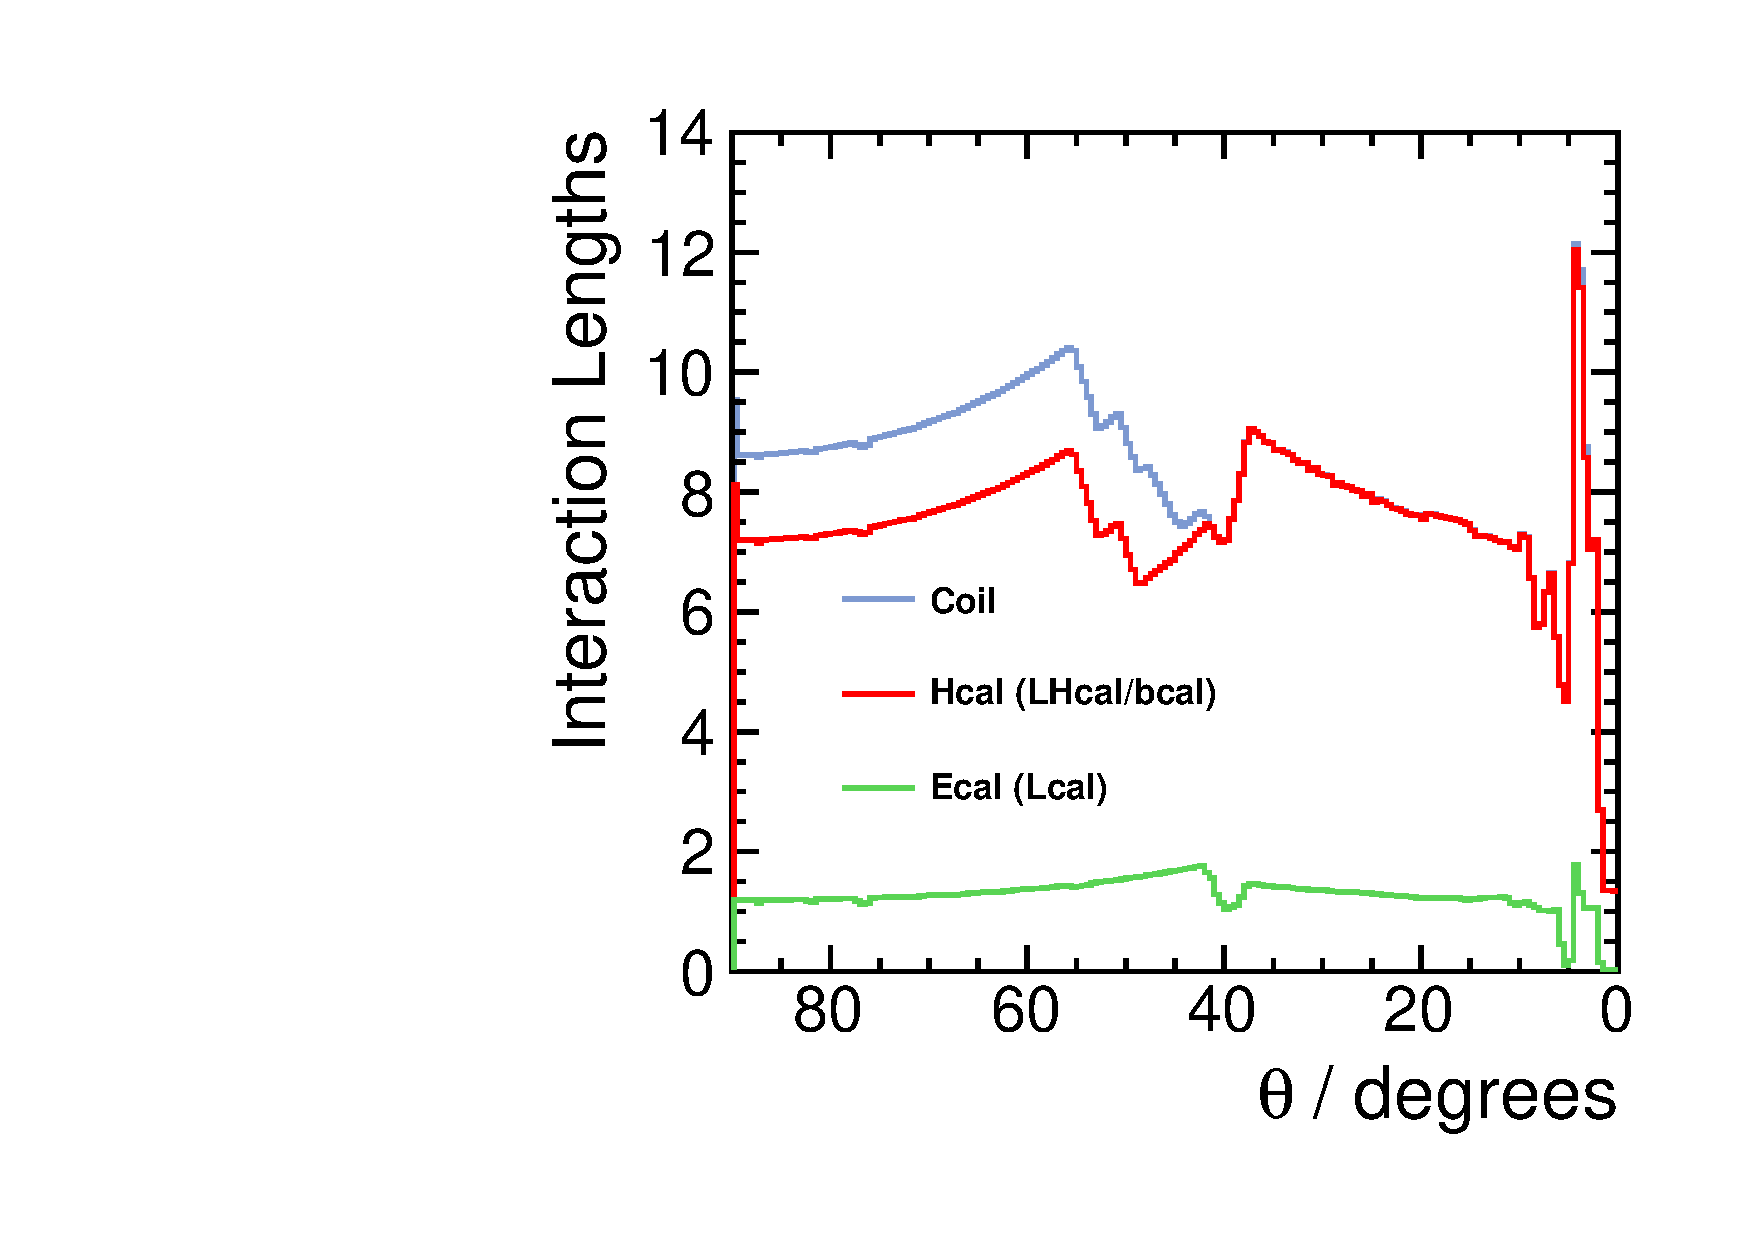
\includegraphics[width=0.5\hsize]{Introduction/fig/intlen_ILD_o1_v05.pdf}
\end{tabular}
\caption[Material in the ILD detector]{Left: Average total radiation length of the material
  in the tracking detectors as a function of polar angle. Right: Total interaction length in the detector, up to the end of the calorimeter system, and including the coil of the detector.}
%\end{figure}
\label{fig:intro:material}
%\begin{tabular}{cc}

\end{figure}

This is followed by a segmented hadronic calorimeter (HCAL) with up to 48 longitudinal samples and small transverse cell size. Two 
options are considered, both based on a Steel-absorber structure. One option uses scintillator tiles of $3 \times 3$\,cm$^2$, 
which are read out with an analogue system. The second uses a gas-based readout which allows a $1 \times 1$\,cm$^2$ 
cell geometry with a semi-digital readout of each cell. 

At very forward angles, below the coverage provided by the ECAL and the HCAL, a system of high precision and radiation hard calorimetric detectors (LumiCAL, BeamCAL, LHCAL) is foreseen. These
extend the calorimetric coverage to almost $4\pi$, measure the luminosity, and  monitor the quality of the colliding beams.

A large volume superconducting coil surrounds the calorimeters, creating an axial $B$-field of nominally 3.5-4\,Tesla.

An iron  yoke, instrumented with scintillator strips or resistive plate chambers (RPCs), returns the magnetic flux of the solenoid, and, at the same time, serves as a muon filter, muon detector and tail catcher calorimeter.

\thisfloatsetup{floatwidth=\SfigwFull,capposition=beside}
\begin{figure}[b!]
\begin{tabular}{cc}

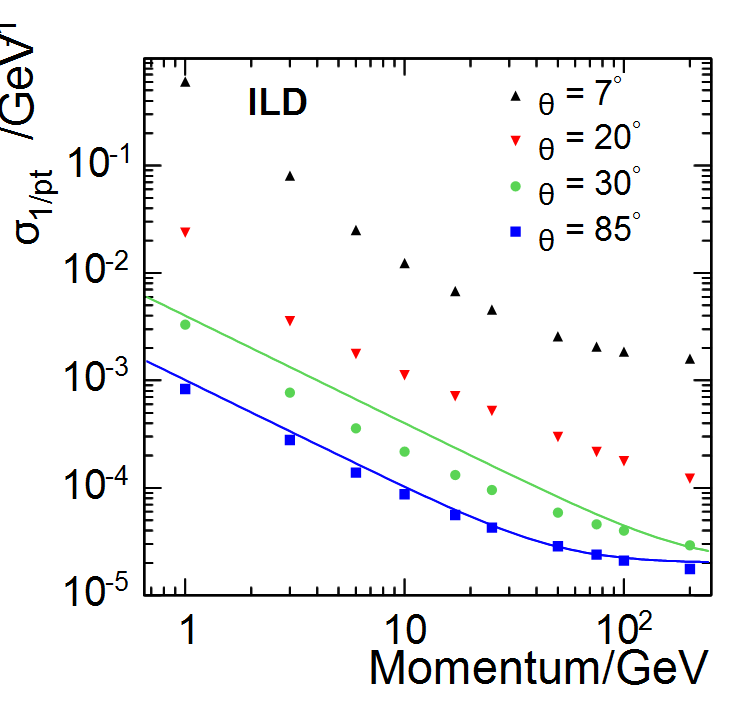
\includegraphics[width=0.5\hsize]{Introduction/fig/deltaInvP_all_fits.png} &
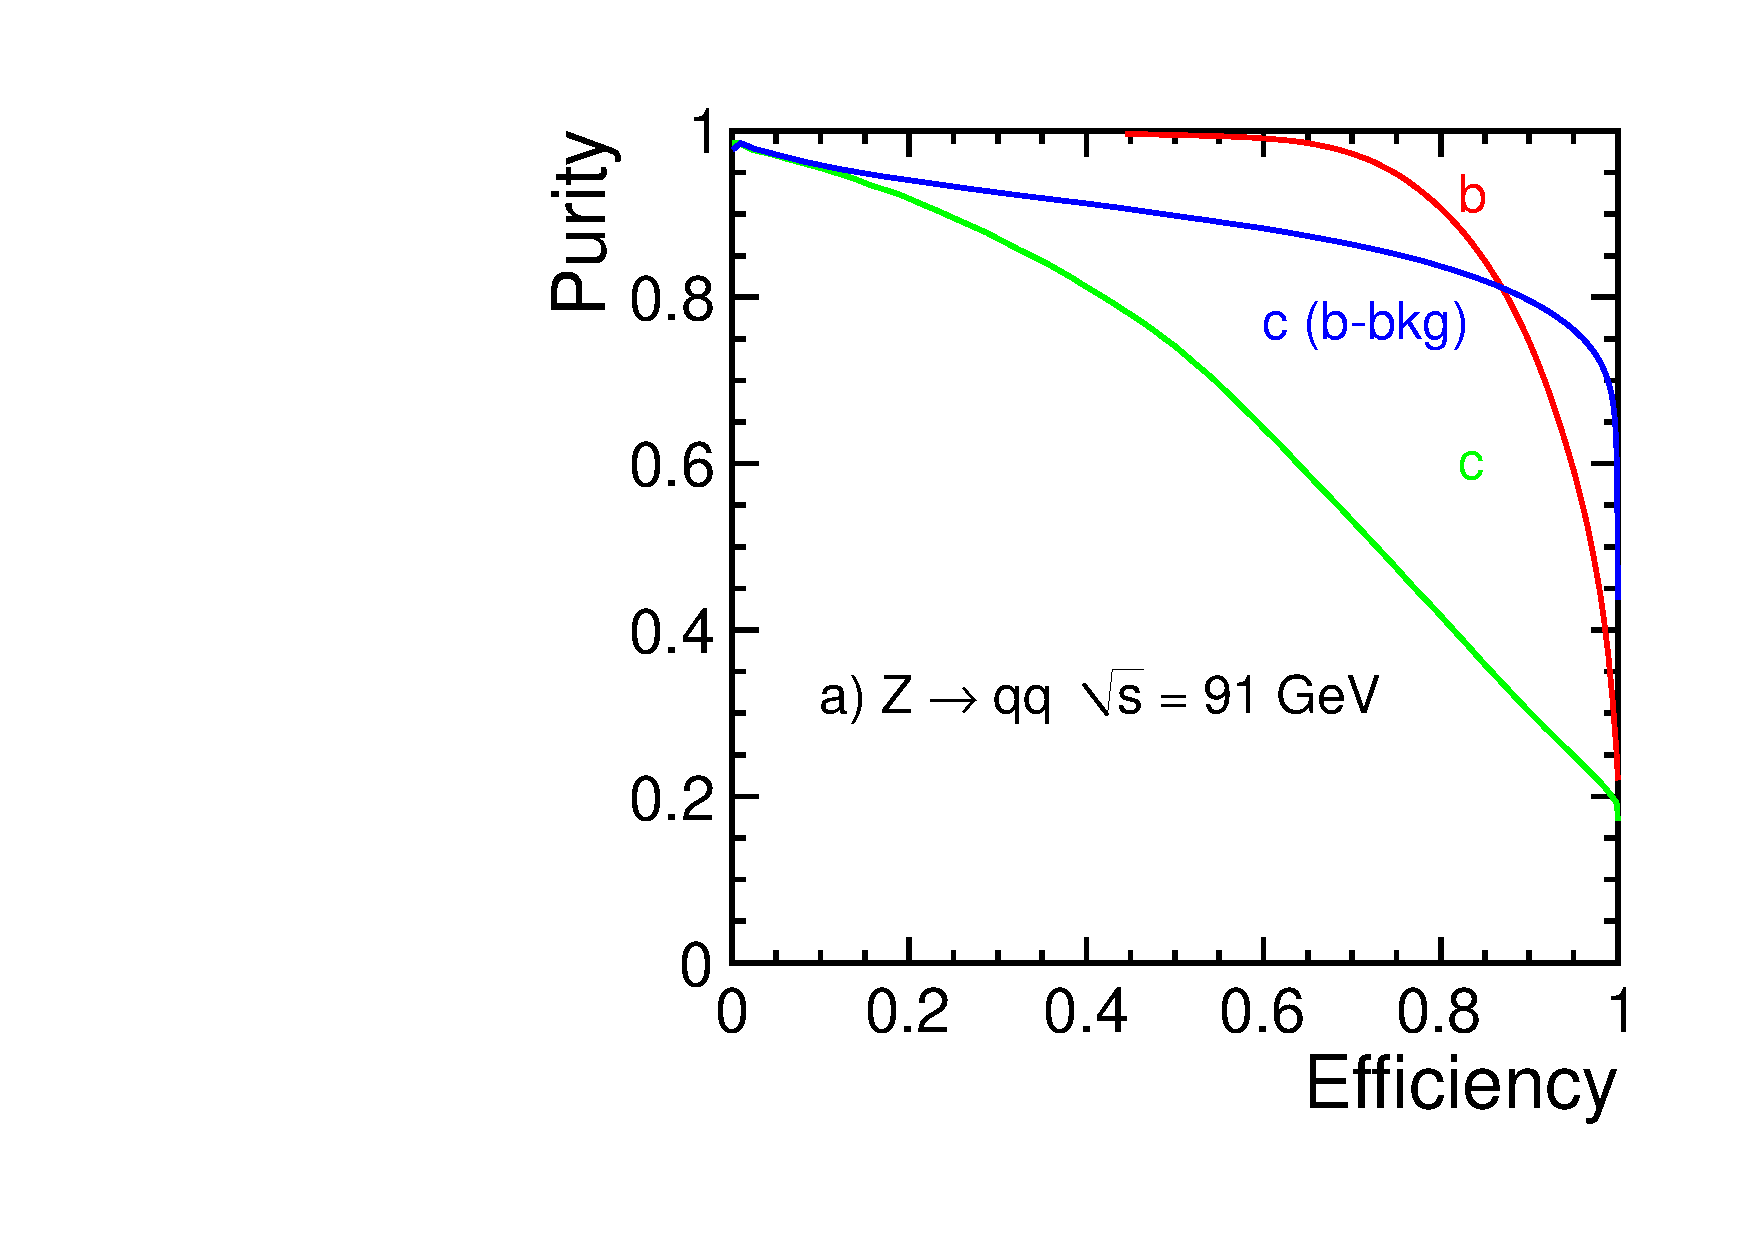
\includegraphics[width=0.5\hsize]{Introduction/fig/evalZ-lcfiweights_qq91new_v02-test.pdf}
\end{tabular}
\caption{\label{ild:fig:intro:tracking}(left) Momentum resolution for the ILD detector concept, as a function of the transverse momentum of the particle. (right) Flavour tagging efficiency versus purity for bottom events in sample of Z decays at 91\,GeV, and for charm events with only bottom background. )}
\end{figure}



\begin{figure}[t!]

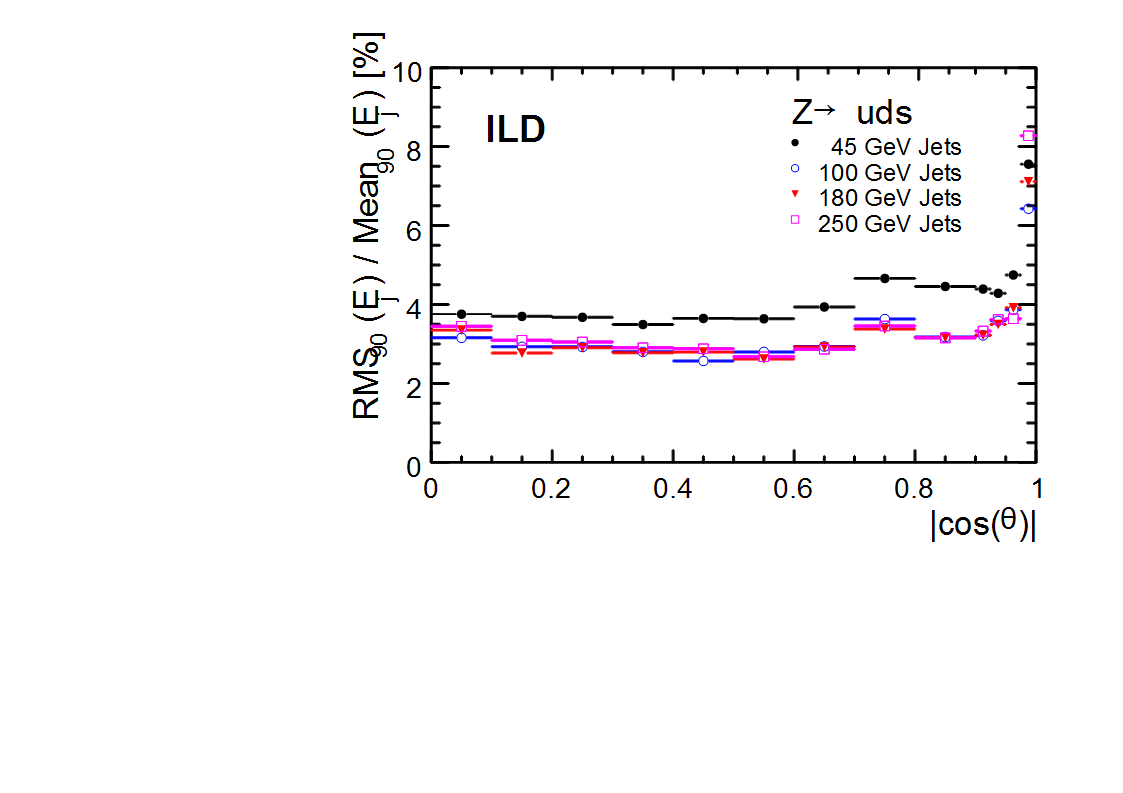
\includegraphics[width=0.8\hsize]{Introduction/fig/ild01_o1_pflow.png}

\caption{\label{ild:fig:intro:pflow}Fractional jet energy resolution
    plotted against $|\cos\theta|$ where theta is the polar angle of the thrust axis of the event. }
\end{figure}

%The main parameters of the ILD detector are summarised in Table~\ref{ild:tab:barrelpara} and table~\ref{ild:tab:endcappara}.
%\begin{sidewaystable}[thb]


The performance of the ILD concept has been extensively studied using a detailed GEANT4 based simulation model and sophisticated reconstruction tools. Backgrounds have been taken into account to the best of current knowledge. 

the key technologies proposed for the ILD detector have been developed in close cooperation with R\&D collaborations and have been extensively tested. The performance numbers of key systems are based on results from prototypes, whereever possible, and extraploated to the full detector performance. This strong check against experimental results ensures that the performance numbers are reliable and are considered a realistic estimate of the ultimate detector performance. 


A key characteristics of the detector is the amount of material in the detector. Particle flow requires a thin tracker, to minimise interactions before the calorimeters, and thick calorimeters, to fully absorb the showers. Figure~\ref{ild:fig:intro:material}~(left) shows the material in the detector in radiation lengths, until the entry of the calorimeter. The right plot shows the total interaction length including the calorimeter system. 

The performance of the tracking system can be summarised by its combined momentum resolution, shown in Figure~\ref{ild:fig:intro:tracking}~(left). A resolution of $\sigma_{1/p_T} = 2 \times 10^{-5}$\,GeV$^{-1}$ has been achieved for high momenta. For many physics studies the tagging of long lived particles is of key importance. Several layers of pixel detectors close to the IP allow the reconstruction of displaced vertices, as shown in Figure~\ref{ild:fig:intro:tracking}~(right).




Calorimeter system and tracking system together enter into the particle flow performance. The performance of the ILD detector for different energies and as a function of the polar angle is shown in Figure~\ref{ild:fig:intro:pflow}. 

The few plots shown in this section illustrate the anticipated performance of the detector and illustrate the potential for precision measurements with the ILD detector. 
